\documentclass[11pt,a4paper]{article}

\usepackage[a4paper,left=2.0cm,right=2.0cm,top=1.55cm,bottom=1.55cm]{geometry}
\usepackage[T1]{fontenc}
\usepackage{lmodern}
\usepackage{graphicx}
\usepackage{xcolor}
\usepackage{array}
\usepackage{tabularx}
\usepackage{ragged2e}
\usepackage{enumitem}
\usepackage{fancyhdr}
\usepackage{tikz}
\usepackage{setspace}
\usepackage{amsmath}

% -------------------------------------------------
% COLOURS
% -------------------------------------------------

\definecolor{TitleBlue}{RGB}{61,103,154}

% -------------------------------------------------
% GENERAL SETTINGS
% -------------------------------------------------

\setlength{\parindent}{0pt}
\setlength{\parskip}{0pt}
\renewcommand{\arraystretch}{1.0}

\newcommand{\blueheading}[1]{%
    {\sffamily\color{TitleBlue}\fontsize{15}{18}\selectfont #1}%
}

\newcommand{\bluebigheading}[1]{%
    {\sffamily\color{TitleBlue}\fontsize{16}{19}\selectfont #1}%
}

\newcommand{\instruction}[1]{%
    {\fontsize{10.5}{12.5}\selectfont #1}%
}

% Content-sized answer box
\newcommand{\answerbox}[1]{%
    \vspace{3pt}
    \noindent
    \fbox{%
        \begin{minipage}{\dimexpr\textwidth-2\fboxsep-2\fboxrule\relax}
            \vspace{1mm}
            \fontsize{13}{15}\selectfont
            #1
            \vspace{1mm}
        \end{minipage}
    }
}

% -------------------------------------------------
% HEADER / FOOTER
% -------------------------------------------------

\pagestyle{fancy}
\fancyhf{}

\renewcommand{\headrulewidth}{0pt}
\renewcommand{\footrulewidth}{0pt}

\fancyhead[L]{%
    \sffamily\bfseries\itshape\fontsize{10.5}{12}\selectfont
    DSCPP-III-2026-T229
}

\fancyhead[R]{%
    \sffamily\bfseries\fontsize{10.5}{12}\selectfont
    PROJECT PROPOSAL
}

\fancyfoot[R]{%
    \itshape\fontsize{10}{12}\selectfont
    Page \thepage
}

\setlength{\headheight}{14pt}
\setlength{\headsep}{23pt}
\setlength{\footskip}{24pt}

% -------------------------------------------------
% DOCUMENT
% -------------------------------------------------

\begin{document}

% =================================================
% PAGE 1
% =================================================

\vspace*{4mm}

\bluebigheading{PROJECT AND TEAM INFORMATION}

\vspace{13mm}

\blueheading{Project Title}

\vspace{1mm}

\instruction{(Try to choose a catchy title. Max 20 words).}

\answerbox{
{MemDB: In-Memory Key-Value Cache}
}

\vspace{13mm}

\blueheading{Student / Team Information}

\vspace{2mm}

\noindent
\begin{tabularx}{\textwidth}
{|>{\RaggedRight\arraybackslash}p{0.69\textwidth}
 |>{\RaggedRight\arraybackslash}X|}
\hline

\begin{minipage}[t]{\linewidth}
\vspace{1.5mm}
\textit{Team Name:}\\[-1mm]
\textit{Team \#}
\vspace{1.5mm}
\end{minipage}
&
\begin{minipage}[t]{\linewidth}
\vspace{1.5mm}
\textit{Epoch}
\vspace{1.5mm}
\end{minipage}
\\
\hline

\begin{minipage}[t][3.25cm][t]{\linewidth}
\vspace{1.5mm}
\textbf{Team member 1 (Team Lead)}\\[-1mm]
\textit{(Last Name, name: student ID: email, picture):}
\vspace{2.0cm}
\end{minipage}
&
\begin{minipage}[t][3.25cm][t]{\linewidth}
\vspace{1.5mm}
\textit{Rawat, Arnav 9068941214}\\
\textit{2510380192@geu.ac.in}

\vspace{2mm}
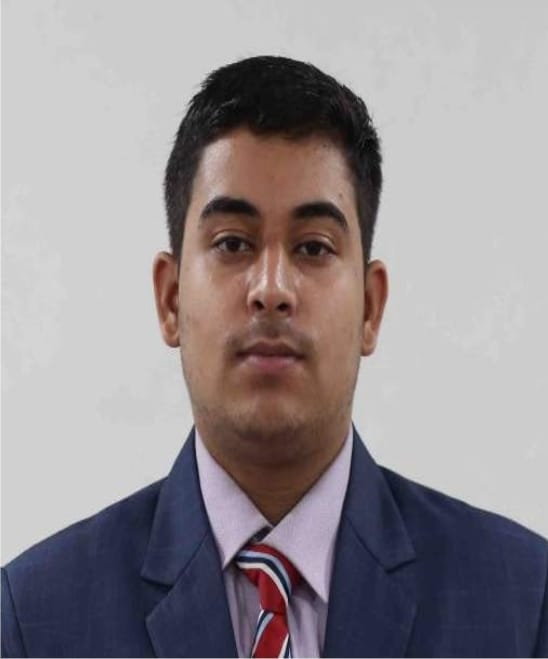
\includegraphics[width=3.0cm,height=1.5cm,keepaspectratio]{member1.png}
\end{minipage}
\\
\hline

\begin{minipage}[t][3.25cm][t]{\linewidth}
\vspace{1.5mm}
\textbf{Team member 2}\\[-1mm]
\textit{(Last Name, name: student ID: email, picture):}
\vspace{2.0cm}
\end{minipage}
&
\begin{minipage}[t][3.25cm][t]{\linewidth}
\vspace{1.5mm}
\textit{Mandal, Anish 7596944379}\\
\textit{2510010615@geu.ac.in}

\vspace{2mm}
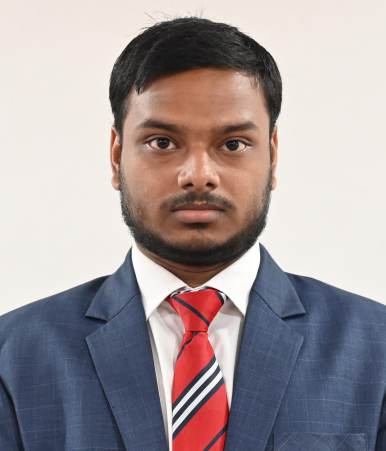
\includegraphics[width=3.0cm,height=1.5cm,keepaspectratio]{member2.png}
\end{minipage}
\\
\hline

\begin{minipage}[t][3.25cm][t]{\linewidth}
\vspace{1.5mm}
\textbf{Team member 3}\\[-1mm]
\textit{(Last Name, name: student ID: email, picture):}
\vspace{2.0cm}
\end{minipage}
&
\begin{minipage}[t][3.25cm][t]{\linewidth}
\vspace{1.5mm}
\textit{Rawat, Suhani 9520955384}\\
\textit{2510387319@geu.ac.in}

\vspace{2mm}
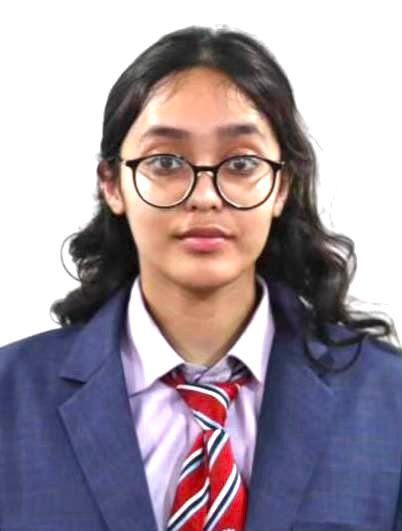
\includegraphics[width=3.0cm,height=1.5cm,keepaspectratio]{member3.png}
\end{minipage}
\\
\hline

\begin{minipage}[t][3.25cm][t]{\linewidth}
\vspace{1.5mm}
\textbf{Team member 4}\\[-1mm]
\textit{(Last Name, name: student ID: email, picture):}
\vspace{2.0cm}
\end{minipage}
&
\begin{minipage}[t][3.25cm][t]{\linewidth}
\vspace{1.5mm}
\textit{Semwal, Priyanshi 9548428370}\\
\textit{2510011737@geu.ac.in}

\vspace{2mm}
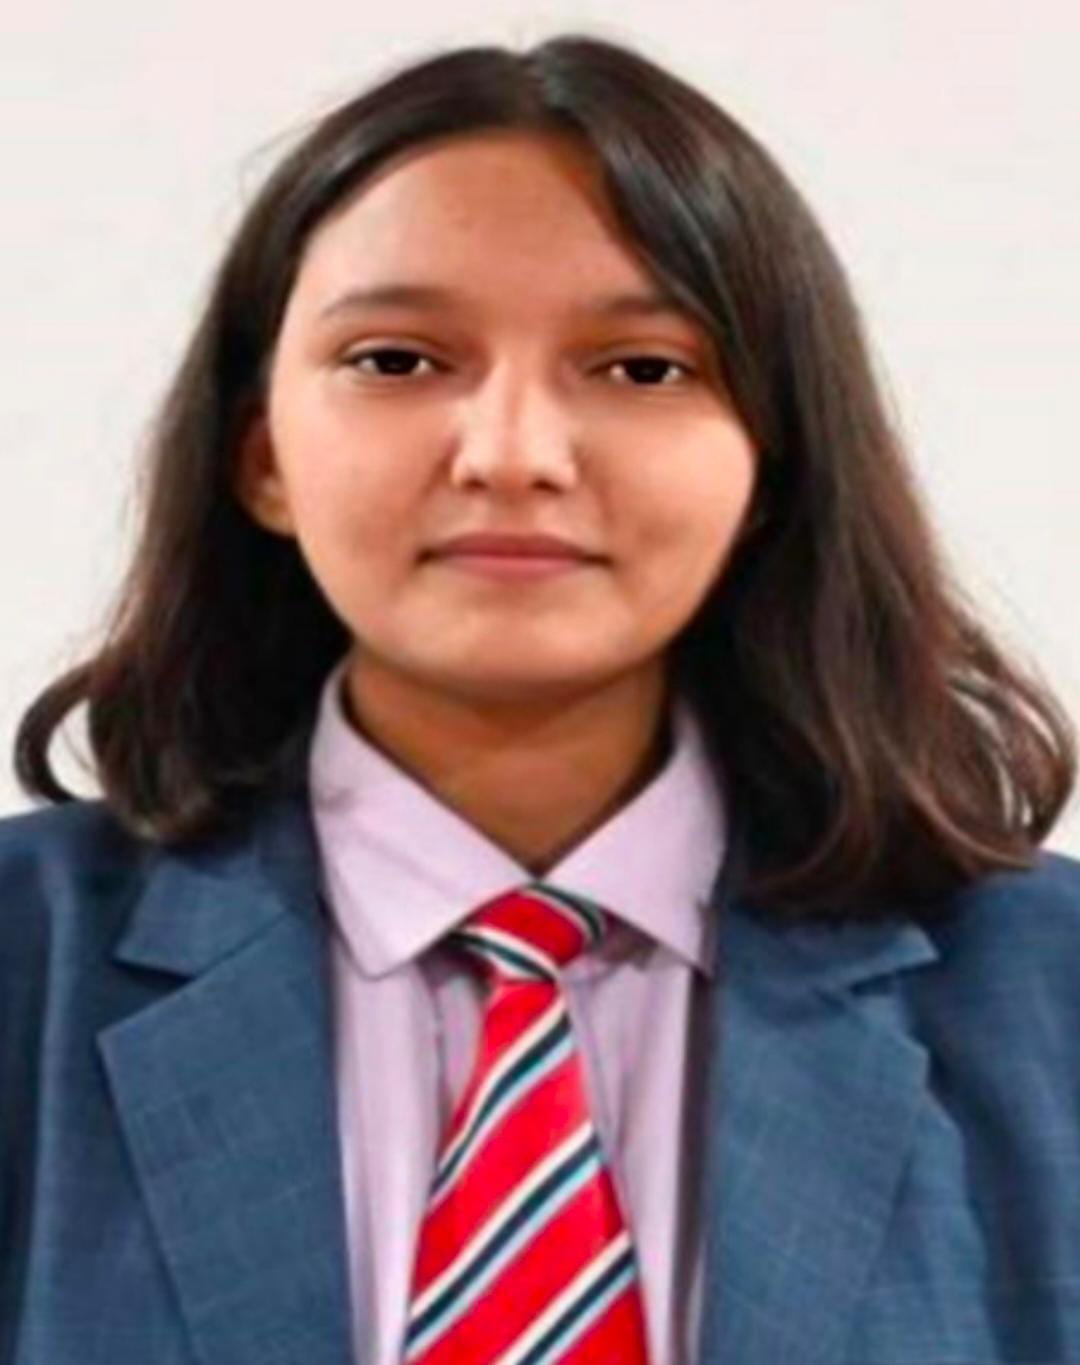
\includegraphics[width=3.0cm,height=1.5cm,keepaspectratio]{member4.png}
\end{minipage}
\\
\hline

\end{tabularx}

\newpage

% =================================================
% PAGE 2
% =================================================

\bluebigheading{PROPOSAL DESCRIPTION (10 pts)}

\vspace{12mm}

\blueheading{Motivation (1 pt)}

\vspace{1mm}

\instruction{(Describe the problem you want to solve and why it is important. Max 300 words).}

\answerbox{
Applications often access the same data repeatedly, even when that data changes infrequently. Retrieving such data repeatedly from a slower backing store can introduce unnecessary latency and additional backend operations. MemDB addresses this problem by providing a lightweight, application-level in-memory key-value cache for temporary and reconstructible data.

The project focuses on demonstrating how appropriate data structures and cache policies can improve repeated data access while operating within a bounded memory budget. MemDB supports key-based lookup, configurable capacity, TTL-based expiration, and multiple eviction policies.

The project also provides an opportunity to study the practical behavior of fundamental data structures under realistic cache operations and evaluate their effectiveness using measurable metrics such as cache hit rate, latency, eviction count, memory usage, and throughput.
}

\vspace{10mm}

\blueheading{State of the Art / Current solution (1 pt)}

\vspace{1mm}

\instruction{(Describe how the problem is solved today (if it is). Max 200 words).}

\answerbox{
Caching is commonly used as an application-level optimization to reduce repeated access to slower data sources. In-memory caches maintain frequently accessed data in RAM and use eviction policies such as LRU or FIFO when their capacity is reached. TTL mechanisms are also commonly used when cached data should remain valid only for a specified period.

MemDB implements these fundamental caching concepts as a compact embedded system. The core data structures remain within the application, providing explicit control over capacity, eviction, expiration, memory accounting, and statistics.

The project is intended primarily as an educational and experimental implementation that allows the behavior of the underlying algorithms and data structures to be visualized and benchmarked.
}

\vspace{10mm}

\blueheading{Project Goals and Milestones (2 pts)}

\vspace{1mm}

\instruction{(Describe the project general goals. Include initial milestones as well any other milestones. Max 300 words).}

\answerbox{
The primary goal is to implement a functional lightweight in-memory key-value cache while demonstrating fundamental data structures, algorithms, and object-oriented programming.

\textbf{Initial milestones:}

\begin{itemize}[leftmargin=*,nosep]
    \item Implement the hash table with collision handling using linked lists.
    \item Implement the doubly linked list required for LRU ordering.
    \item Implement a custom min-heap for TTL expiration management.
    \item Implement SET, GET, DELETE and CLEAR operations.
    \item Implement both LRU and FIFO eviction policies.
    \item Implement configurable memory capacity and memory usage tracking.
    \item Implement cache statistics including hits, misses and evictions.
    \item Build the C++ interface and policy abstraction using OOP.
    \item Develop a GUI for cache interaction and visualization.
    \item Implement benchmarking for progressively larger workloads.
\end{itemize}

The final milestone is an integrated demonstration showing insertion, lookup, collision handling, rehashing, LRU movement, eviction, TTL expiration, memory usage, statistics, and performance measurements.
}

\vspace{8mm}

\blueheading{Project Approach (3 pts)}

\vspace{1mm}

\instruction{(Describe how you plan to articulate and design a solution. Including platforms and technologies that you will use. Max 300 words).}

\answerbox{
MemDB is designed as a layered system that separates the core data structures from cache management and the GUI.

The low-level data-structure layer is implemented in \textbf{C}. A hash table provides average $O(1)$ key-based lookup with linked-list collision handling. A doubly linked list maintains ordering information required by LRU eviction. A custom min-heap maintains expiration times so that the earliest expiring entry can be identified efficiently.

The higher-level cache management layer is implemented in \textbf{C++}. Classes encapsulate cache entries, cache management, statistics, memory accounting, and eviction policies. LRU and FIFO policies are represented through an object-oriented policy interface, allowing the eviction strategy to be selected without changing the core storage implementation.

The cache maintains a configurable memory limit and tracks used and available memory. When capacity is exceeded, the selected eviction policy removes entries according to its rules. TTL expiration is managed using the expiration min-heap.

A GUI provides interactive visualization of cache contents, statistics, memory usage, the selected eviction policy, and the internal data structures. The system is intended to run as a desktop application using C and C++.

Finally, benchmarking will measure latency, throughput, cache hit rate, evictions, memory consumption, and performance as dataset size increases.
}

\newpage

% =================================================
% PAGE 3
% =================================================

\blueheading{System Architecture (High Level Diagram)(2 pts)}

\vspace{1mm}

\instruction{(Provide an overview of the system, identifying its main components and interfaces in the form of a diagram using a tool of your choice).}

\vspace{5mm}

\begin{center}

\begin{tikzpicture}[
    box/.style={
        draw,
        rounded corners=3pt,
        align=center,
        minimum width=4.2cm,
        minimum height=0.8cm,
        font=\small
    },
    component/.style={
        draw,
        rounded corners=3pt,
        align=center,
        minimum width=3.2cm,
        minimum height=0.75cm,
        font=\small
    },
    arrow/.style={
        ->,
        thick
    }
]

% GUI
\node[box] (gui) at (0,0)
{GUI / Visualization};

% C++ layer
\node[box] (cpp) at (0,-1.5)
{C++ MemDB Management Layer};

\node[component] (policy) at (-3,-2.9)
{Eviction Policies\\LRU / FIFO};

\node[component] (stats) at (3,-2.9)
{Statistics \&\\Memory Manager};

% C layer
\node[box] (clayer) at (0,-4.3)
{C Data-Structure Layer};

\node[component] (hash) at (-4,-5.8)
{Hash Table\\+ Collision Lists};

\node[component] (list) at (0,-5.8)
{Doubly Linked List};

\node[component] (heap) at (4,-5.8)
{Min-Heap\\TTL Expiration};

% Memory
\node[box] (memory) at (0,-7.4)
{In-Memory Cache};

% Connections
\draw[arrow] (gui) -- (cpp);

\draw[arrow] (cpp) -- (policy);
\draw[arrow] (cpp) -- (stats);

\draw[arrow] (policy) -- (clayer);
\draw[arrow] (stats) -- (clayer);

\draw[arrow] (clayer) -- (hash);
\draw[arrow] (clayer) -- (list);
\draw[arrow] (clayer) -- (heap);

\draw[arrow] (hash) -- (memory);
\draw[arrow] (list) -- (memory);
\draw[arrow] (heap) -- (memory);

\end{tikzpicture}

\end{center}

\vspace{5mm}

\textbf{Operational flow:}

\begin{center}
\small
GUI
$\rightarrow$
C++ MemDB API
$\rightarrow$
C Data Structures
$\rightarrow$
In-Memory Cache
\end{center}

\vspace{3mm}

\textit{The C layer implements the core data structures, while the C++ layer manages cache policies, statistics, memory accounting, and interaction with the GUI.}

\vspace{10mm}

\blueheading{Project Outcome / Deliverables (1 pts)}

\vspace{1mm}

\instruction{(Describe what are the outcomes / deliverables of the project. Max 200 words).}

\answerbox{
The primary deliverable is a working MemDB prototype implementing an in-memory key-value cache with configurable capacity, LRU and FIFO eviction policies, TTL-based expiration, memory tracking, and cache statistics.

The project will include the C implementation of the hash table, collision-handling lists, doubly linked list, and custom min-heap. The C++ layer will provide the object-oriented cache interface, eviction-policy abstraction, statistics management, and memory management.

A GUI will demonstrate cache contents, memory usage, statistics, selected eviction policy, and internal data-structure behavior. The system will provide interactive demonstrations of collision handling, rehashing, LRU movement, eviction, and TTL expiration.

Benchmark results will report performance for progressively larger workloads and compare the observed behavior with the expected algorithmic complexity.
}

\vspace{9mm}

\blueheading{Assumptions}

\vspace{1mm}

\instruction{(Describe the assumptions (if any) you are making to solve the problem. Max 100 words).}

\answerbox{
MemDB operates as an application-level cache for temporary or reconstructible data and does not replace persistent storage. The initial prototype operates primarily in memory within a single process. Persistence, networking, distributed synchronization, and multithreading are outside the core scope. Cache entries are assumed to have manageable key and value sizes, while the configured memory limit is assumed to be sufficient for the intended workloads. TTL values are based on the system clock.
}

\vspace{9mm}

\blueheading{References}

\vspace{1mm}

\instruction{(Provide a list of resources or references you utilised for the completion of this deliverable. You may provide links).}

\answerbox{
\begin{enumerate}[leftmargin=*,nosep]
    \item Thomas H. Cormen, Charles E. Leiserson, Ronald L. Rivest and Clifford Stein, \textit{Introduction to Algorithms}, MIT Press.

    \item Brian W. Kernighan and Dennis M. Ritchie, \textit{The C Programming Language}, Prentice Hall.

    \item Bjarne Stroustrup, \textit{The C++ Programming Language}, Addison-Wesley.
\end{enumerate}
}

\end{document}